\documentclass[../../time_series_notes.tex]{subfiles}
\begin{document}
%%%%%%%%%%%%%%%%%%%%%%%%%%%%%%%%%%%%%%%%%%%%%%%%%%%%%%%%%%%%
\section{Exponential Smoothing with Trend and Seasonality}
Also known as \textbf{Holt-Winter's Method} and \textbf{Triple Exponential Smoothing}, this method extends the double exponential smoothing method to add seasonality component/seasonality smoothing as well. The seasonal component can be added in two ways
\begin{itemize}
    \item Additive: The seasonal component stays constant with the level of series
    \item Multiplicative: The seasonal component grows with the level of the series.
\end{itemize}

\subsection{Additive Model for Seasonality}
Let $m$ denote the seasonality of the data. The additive model for seasonality is
\begin{align*}
    x_{t+h|t} &= l_{t} + h\beta b_{t} + s_{t+h - m(k+1)}, \quad k = \lfloor \frac{h-1}{m} \rfloor\\
    l_{t} &= \alpha(x_{t-1} - s_{t-m}) + (1-\alpha)(l_{t-1} + b_{t-1})\\
    b_{t} &= \beta (l_{t} - l_{t-1}) + (1-\beta)b_{t-1}\\
    s_{t} &= \gamma(x_{t} - l_{t-1}-b_{t-1}) + (1-\gamma)s_{t-m}
\end{align*}
where the level smoothing equation adjusts $x_{t-1}$ to remove the seasonal component and averages this value with the non seasonal forecast $l_{t-1} + b_{t-1}$. Trend equation is same as double exponential smoothing, and seasonal component equation averages the current seasonal component (remove trend and level from current time series) with seasonal component $m$ cycles back. Also, $\alpha, \beta, \gamma \in [0,1]$. The initial values of different components are often chosen by the program itself during optimization.\newline

Figure shows how the level, trend and seasonality separate for a set of parameters. These are not the optimal values but chosen for illustration. Notice how the trend gives an average view of the series, similar to a moving average filter. Trend and seasonality added on top of level will give the original series.
\begin{figure}[h]
    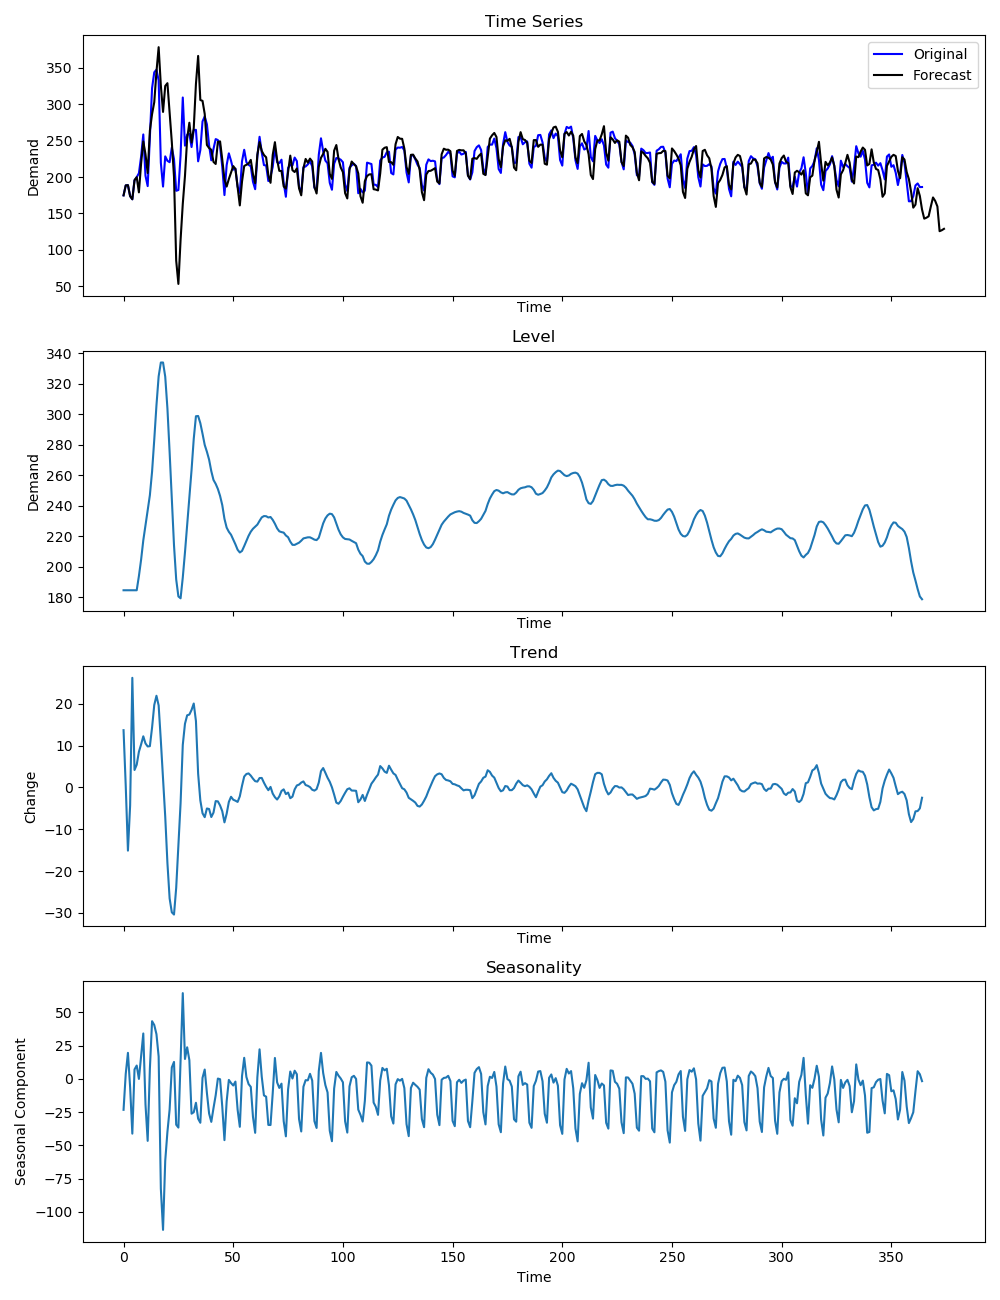
\includegraphics[scale=0.6]{ses_season_1}
    \centering
    \caption {First figure shows the original and forecasted series for $\alpha=0.1, \beta=0.8$ and $\gamma=0.6$. The forecast for future data is downwards linear due to the local trend there. Second, third and fourth figures show the level, trend and seasonal component. The noise in inital part is due to the naive initialization. Figures plot using ses\_season.py}
    \label{fig:ses_season_1} %\ref{fig:ses_season_1}
\end{figure}



\subsection{Multiplicative Model for Seasonality}
The multiplicative seasonality model is similar but instead of additive operations for seasonality, we use multiplicative operations
\begin{align*}
    x_{t+h|t} &= (l_{t} + h\beta b_{t}) s_{t+h - m(k+1)}, \quad k = \lfloor \frac{h-1}{m} \rfloor\\
    l_{t} &= \alpha\frac{x_{t-1}}{s_{t-m}} + (1-\alpha)(l_{t-1} + b_{t-1})\\
    b_{t} &= \beta (l_{t} - l_{t-1}) + (1-\beta)b_{t-1}\\
    s_{t} &= \gamma\frac{x_{t}}{l_{t-1}-b_{t-1}} + (1-\gamma)s_{t-m}
\end{align*}

Similar to last section, we can prepare a damped model for seasonality
\begin{align*}
    x_{t+h|t} &= (l_{t} + (\phi + \phi^{2} + \cdots + \phi^{h})\beta b_{t}) s_{t+h - m(k+1)}, \quad k = \lfloor \frac{h-1}{m} \rfloor\\
    l_{t} &= \alpha\frac{x_{t-1}}{s_{t-m}} + (1-\alpha)(l_{t-1} + \phi b_{t-1})\\
    b_{t} &= \beta (l_{t} - l_{t-1}) + (1-\beta)\phi b_{t-1}\\
    s_{t} &= \gamma\frac{x_{t}}{l_{t-1}-\phi b_{t-1}} + (1-\gamma)s_{t-m}
\end{align*}

It is very important to note that we can keep any combinations of trend, seasonal and dampened smoothing in our model. Level will always be present, but based on our choice of the model, we can play around with the corresponding smoothing equations. For instance, a model without trend will simply ignore all terms related to trend and also ignore the trend equation.

\end{document}